1. zhang code, generated

2. example with lists
3. complex list(add, sub) with focus on updates

\section{Scenario}
\textcite{zhang2019scenario} use an example of a small \gls{spa} titled "Math for kids", which generates simple math addition problems and keeps track of a small statistic, which includes the number of correctly and incorrectly answered problems. The same application has been implemented and extended in Vue.js and will be used to display the capabities of the interaction diagram and scenario generation application.
\section{Math for Kids}

\begin{figure}[H]
    \centering
    \begin{subfigure}[b]{0.45\textwidth}
         \centering
         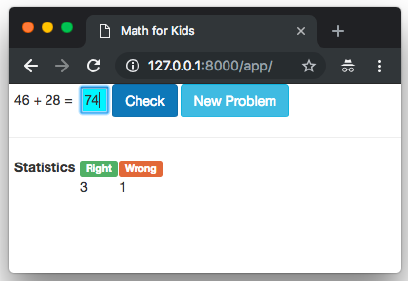
\includegraphics[width=0.45\textwidth]{images/math_for_kids_zhang.png}
         \caption{Math for Kids in AngularJS by \textcite{zhang2019scenario}}
         \label{fig:evaluation_math_kids_zhang}
    \end{subfigure}
    \begin{subfigure}[b]{0.45\textwidth}
        \centering
        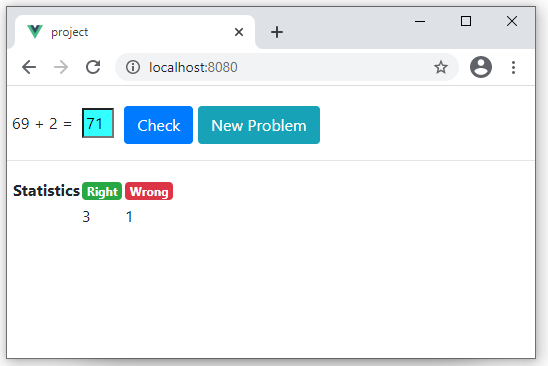
\includegraphics[width=0.45\textwidth]{images/math_for_kids_own.png}
        \caption{Own implementation of Math for Kids in Vue.js}
        \label{fig:evaluation_math_kids_own}
    \end{subfigure}
\end{figure}

The source code can be found in \code{resources/test-files/test.vue} and also in \ref{appendix:math_kids_basic_source_code}.
\begin{figure}[H]
    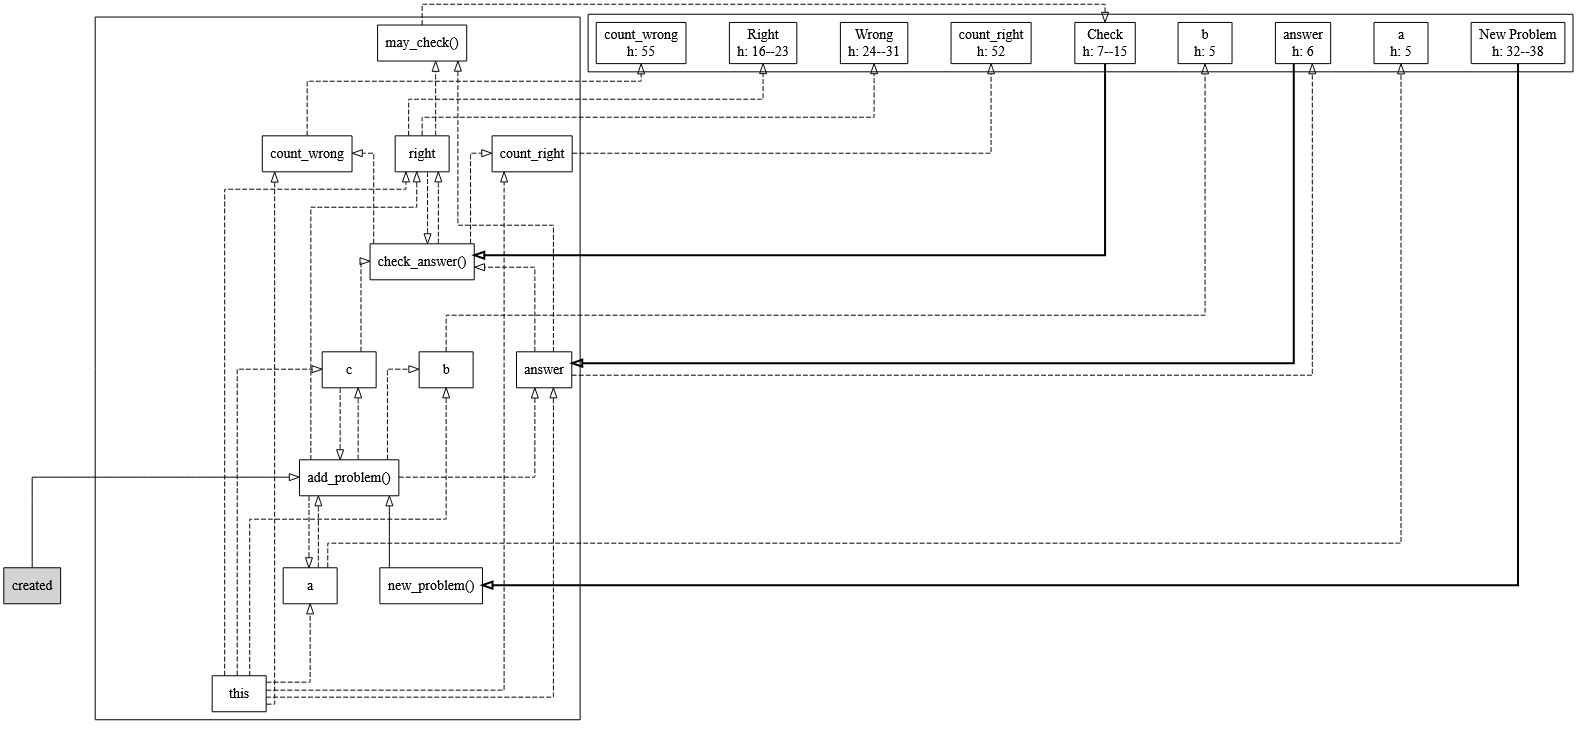
\includegraphics[width=\textwidth]{images/diagram_own_math_kids.png}
     \caption{Math for Kids in Vue.js generated interaction diagram }
     \label{fig:math_for_kids_own_interaction_diagram}
\end{figure}

\begin{figure}[H]
    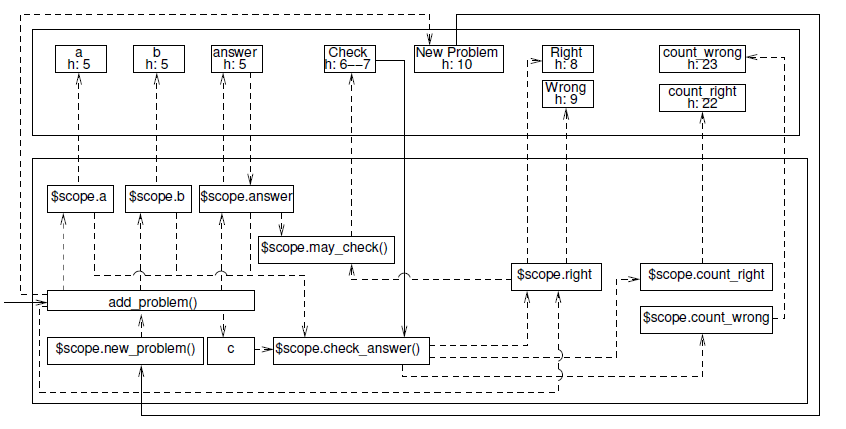
\includegraphics[width=\textwidth]{images/interaction_diagram_zhang.png}
     \caption{Math for Kids in AngularJS interaction diagram by \textcite{zhang2019scenario}}
     \label{fig:math_for_kids_zhang_interaction_diagram}
\end{figure}

When comparing the generated diagram\ref{fig:math_for_kids_own_interaction_diagram} to the original by \textcite{zhang2019scenario} \ref{fig:math_for_kids_zhang_interaction_diagram} there are some differences.

Due to different modelling there is a \code{this} vertex and connections from it to top level variables, which does not exist in the diagram by \textcite{zhang2019scenario}. In the generated diagram there is an edge of type 'event' between the \textit{answer} tag and \textit{answer} property. This is due to the way that two-way bindings were decided to be represented.

There are two differences between the \textit{add\_problem} node in the generated diagram and the one by \textit{zhang2019scenario}.
In \textcite{zhang2019scenario} there is an edge from
the \textit{add\_problem} method to the \textit{New Problem} tag, which is missing in the own generated version. This seems like a mistake in \parencite{zhang2019scenario}, since this edge should not exist.

The other difference is that in \parencite{zhang2019scenario} there is no edges from \textit{add\_problem} to \textit{right} (write relation), however there should be, 
inside \textit{add\_problem} \code{this.right = undefined}.

\begin{lstlisting}
l(created) -> a, b, answer, Check, Right, Wrong
l(answer) -> answer, Check
l(Check) -> Right, Wrong, Check, count_right, count_wrong
l(New Problem) -> a, b, answer, Check, Right, Wrong
\end{lstlisting}

The generated reaction based on the graph differ for $l(created)$, all other sets are exactly the same as the ones by \textcite{zhang2019scenario} (albeit in different order). This may stem from the fact that the edges of \textit{add\_problem} to \code{\$scope.right} is missing in \parencite{zhang2019scenario}, however it is later correctly factored in $l(New Problem)$.

\textcite{zhang2019scenario} define $l(add_problem())$ 
(the equivalent of $l(created)$) as $l(add_problem() = 
{a, b})$ where it should be 
$l(add_problem() = {Check, Right, Wrong, a, b, answer })$ since the answer property is updated based on the diagram. 

One could argue, that the version in \parencite{zhang2019scenario} is correct, since $answer$ is set to $undefined$, which is the same as the initial value of the variable, so it would not trigger an update as part of the \code{init} method. The interaction diagram generator does not perform this check. If $l(add_problem())$ were to be called later in the application (when the $New Problem$ button is clicked) it would indeed set a new value to $answer$, which is correctly reflected by \textcite{zhang2019scenario}.


\subsection{Scenarios}
The following Gherkin scenarios of up to 4 elements are generated. The program outputs this as plain text to the console, but here they are displayed in a nicer way.


\section{Diagram with list}
which can be found in \code{resources/test-files/list.vue}
\begin{figure}[H]
    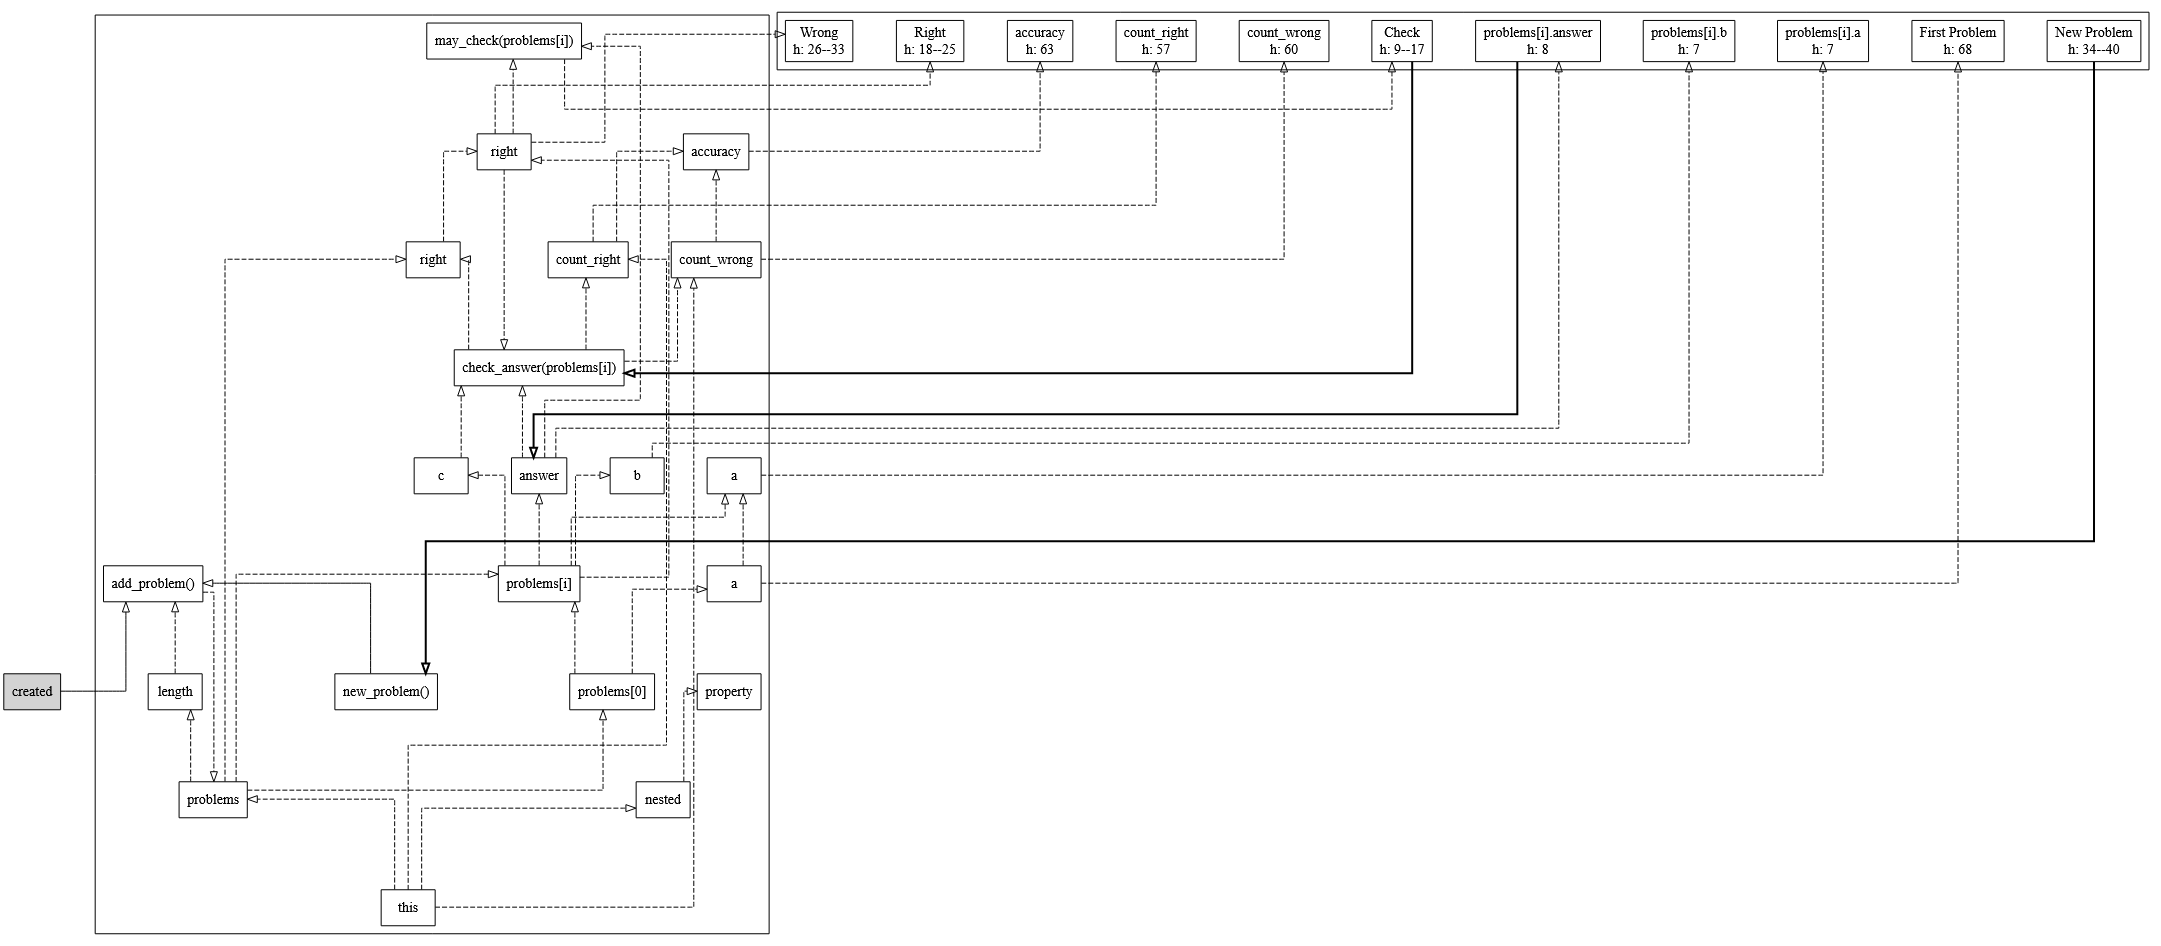
\includegraphics[width=\textwidth]{images/diagram_list.png}
     \caption{TODO}
     \label{fig:diagram_list}
\end{figure}

% \section{Diagram Addition and Substitution}
% \begin{figure}[H]
%     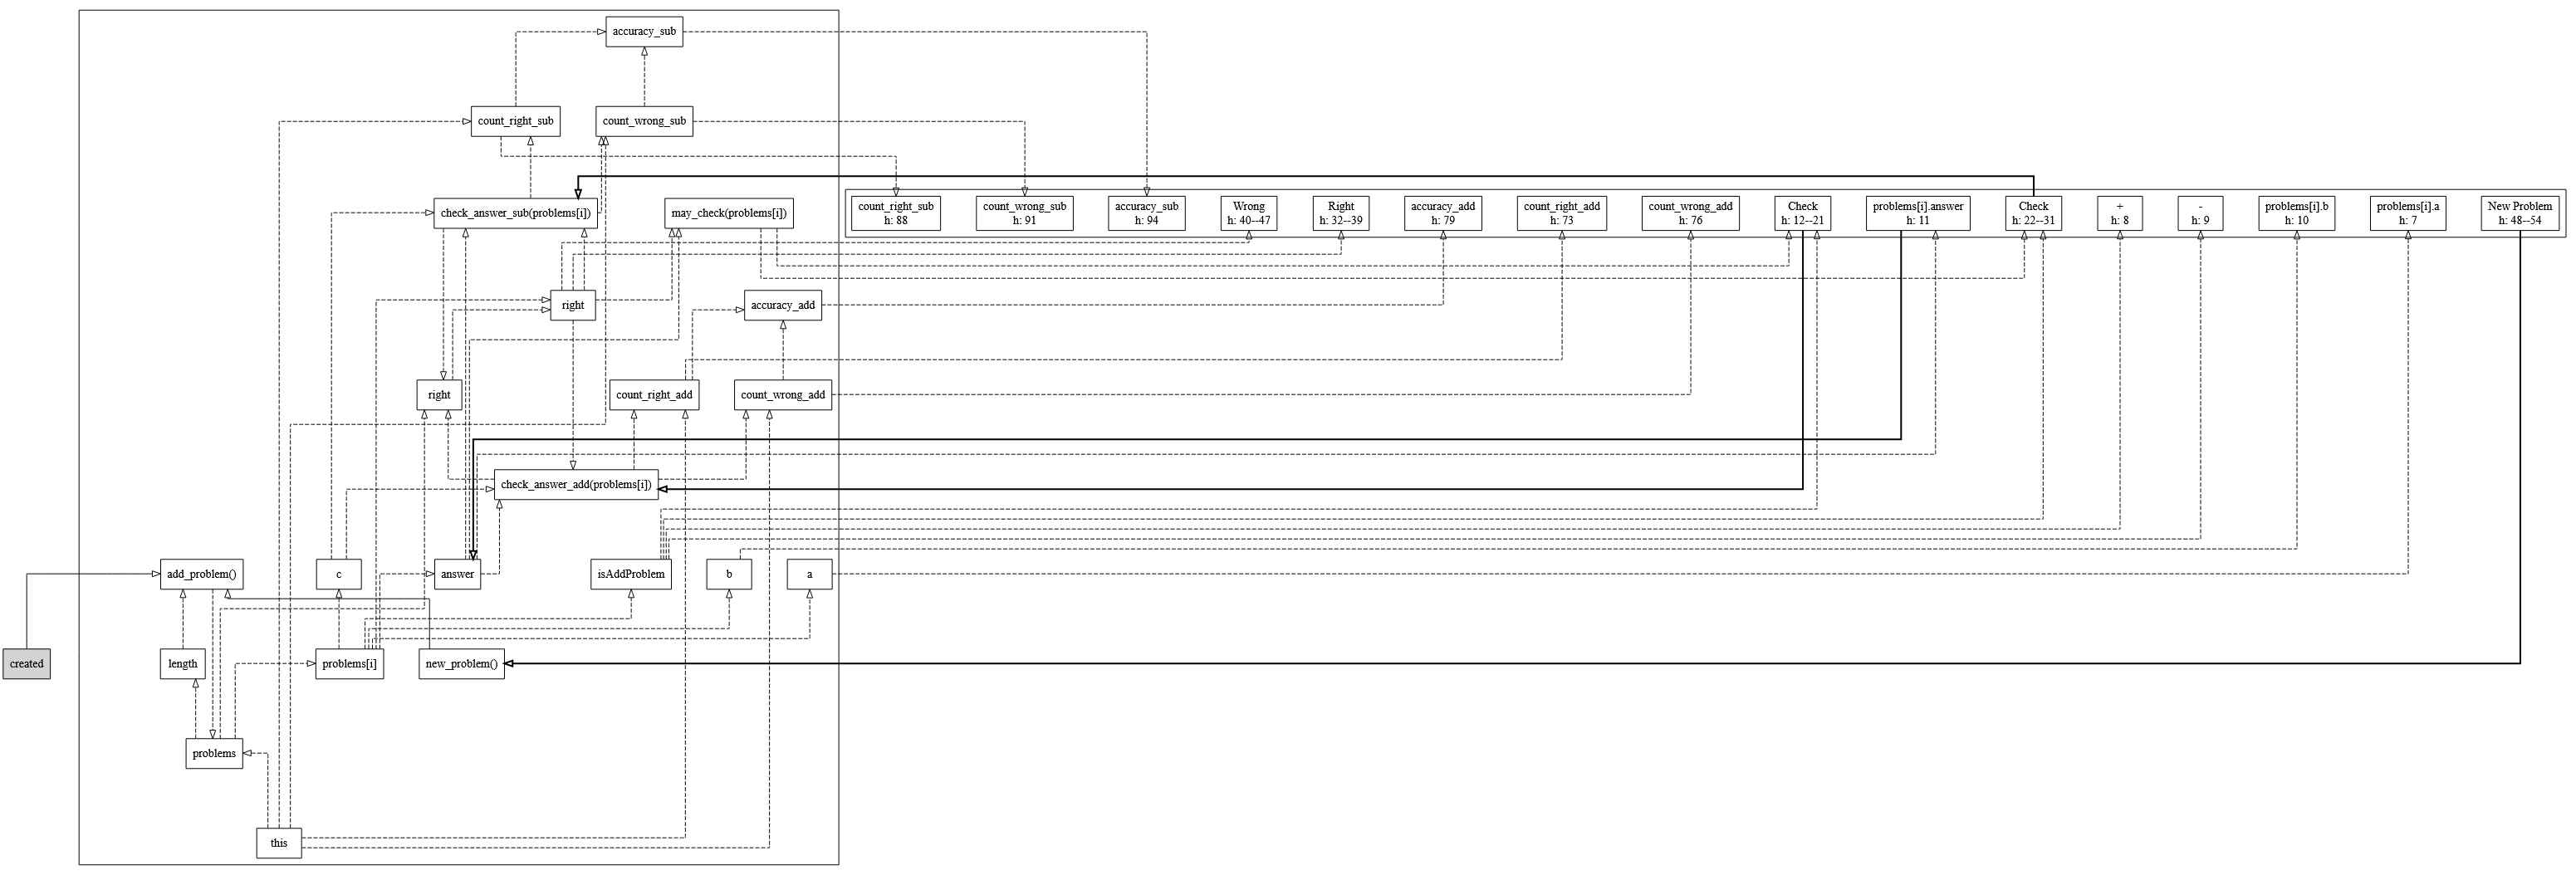
\includegraphics[width=\textwidth]{images/diagram_list_add_sub.png}
%      \caption{TODO }
%      \label{fig:diagram_test_add_sub}
% \end{figure}


%TODO link to https://github.com/KarakoA/vuejs-example and say examples can be deployed there